\section{Results}\label{sec:results}
%\marco{In my opinion, this introduction should go.}
To successfully perform the NA-task, the LSTM-LM should encode and store at least two types of information: (1) the grammatical number of the subject; and (2) syntactic structure of the main subject-verb dependency. The latter information is important for identifying the time period during which the network should store the grammatical-number of the subject and at what time point it should output and update it. This section describes the 'neural circuit' of the LSTM-LM that encodes this type of information required to solve the NA-task.

\subsection{Long-range number-units}\label{subsec:ablation}
\begin{center}
\begin{table}[ht]
\centering
\begin{tabular}{|P{2.3cm}|P{0.4cm}||P{0.6cm}|P{0.6cm}|P{0.6cm}|}
\hline
\B NA task & \B C & \B 776 & \B 988 & \B Full \\
\hline
\hline

% Singular conditions

Simple & S & - &  - &  100 \\

Adv & S & - &  - &  100 \\

2Adv & S & - &  - &  99.9 \\

Co-Adv & S & - &  \textcolor{red}{82} &  98.7 \\

namePP & S & - &  - &  99.3 \\

nounPP & SS & - &  - &  99.2 \\

nounPP & SP &  - &  \textcolor{red}{54.2} &  87.2 \\

nounPP-Adv & SS &  - &  - & 99.5 \\

nounPP-Adv & SP &  - &  \textcolor{red}{54.0} & 91.2 \\


\hline
% Plural conditions
Simple & P &  - &  - &  100 \\

Adv & P &  - &  - &  99.6 \\

2Adv & P & - &  - &  99.3 \\

Co-Adv & P &  \textcolor{blue}{79.2} &  - &  99.3 \\

namePP & P & \textcolor{blue}{39.9} &  - &  68.9 \\

nounPP & PS &  \textcolor{blue}{48.0} & - &  92.0 \\

nounPP & PP &  \textcolor{blue}{78.3} & - &  99.0 \\

nounPPadv & PS & \textcolor{blue}{63.7} &  - &  99.2 \\

nounPPadv & PP & - &  - &  99.8 \\

\hline
\hline
\B Linzen & \B - &  ? &  ? &  ? \\
\hline
\end{tabular}
\caption{Ablation experiments results: Percentage of correct subject-verb agreements in all NA-tasks. Full: non-ablated model, C: condition, S - singular, P - plural. For task with two nouns, SS - singular-singular, SP - singular-plural, PS - plural-singular, PP - plural-plural. Red: Singular subject, Blue: Plural subject. \label{tab:ablation-results}}
\end{table}
\end{center}

We start by describing the behavioral results of the LSTM-LM on the various NA-tasks (section~\ref{sec:the_data}). Network performance on each NA-task is reported in Table 1 (right column - 'Full'). We highlight several aspect of these results. First, some NA-tasks and conditions are clearly more difficult for the network than others. For example, performance on the simple NA-task is better than that on the Co-Adv NA-task, which in turn is better than that of the nounPP tasks. Second, conditions with an interfering noun before the verb (the incongruent conditions of nounPP and nounPPadv) reduce network performance: $ACC_{nounPP-SP}>ACC_{nounPP-SS}$ and $ACC_{nounPP-PS}>ACC_{nounPP-PP}$. Last, for long-range dependencies, reliably encoding singular subject across an interfering noun is more difficult than a plural subject: $ACC_{nounPP-SP}<ACC_{nounPP-PS}$ and $ACC_{nounPPadv-SP}<ACC_{nounPPadv-PS}$ \yair{is it still the case in the results?!}. Interestingly, this singular-plural asymmetry has been reported also in humans. 

\subsubsection{Local vs. distributed code - an ablation study}
Generally, number information may be stored in the network in either a local, sparse, or a distributed way, depending on the fraction of active units that carry number information. 
We hypothesized that if the network uses a local or sparse coding, meaning that there's a small set of units that encode number information, then ablating these units would lead to a drastic decrease in performance on the NA-task, compared to when ablating other units. 
To test this, we conducted ablation experiments in which each time a single unit of the network is ablated and the resulting model is then evaluated on each of the NA-tasks (section 3.1). 

Two units were found to have exceptional effect on network performance (\ref{tab:ablation-results} \unit{2}{126} and \unit{2}{338}. Ablating these units reduced network performance by more than 10\% across various conditions, and importantly, they were the only units whose ablation consistently brought network performance to around chance level in the incongruent conditions of the nounPP and nounPPadv tasks. These conditions are in particular revealing by having a long-range dependency with an interfering noun before the verb. A small subset of other units also had an impact on network performance, but not as dramatically and consistently as that of units \unit{2}{126} and \unit{2}{338} \footnote{\yair{report performance for these other units}}. Importantly, the effect of the ablation depended on the grammatical number of the subject: \unit{2}{126} significantly reduces network performance only if the subject is plural and \unit{2}{338} only if the subject is singular. In what follows, we will therefore refer to these units as a 'plural' and 'singular' units, respectively, or long-range (LR) number units when referring to both. Taken together, these results suggest a highly local coding scheme of grammatical-number required for long-range dependencies. 

\subsubsection{Visualizing gate and cell-state dynamics}\label{subsec:gate-dynamics}
\begin{figure*}[ht]
%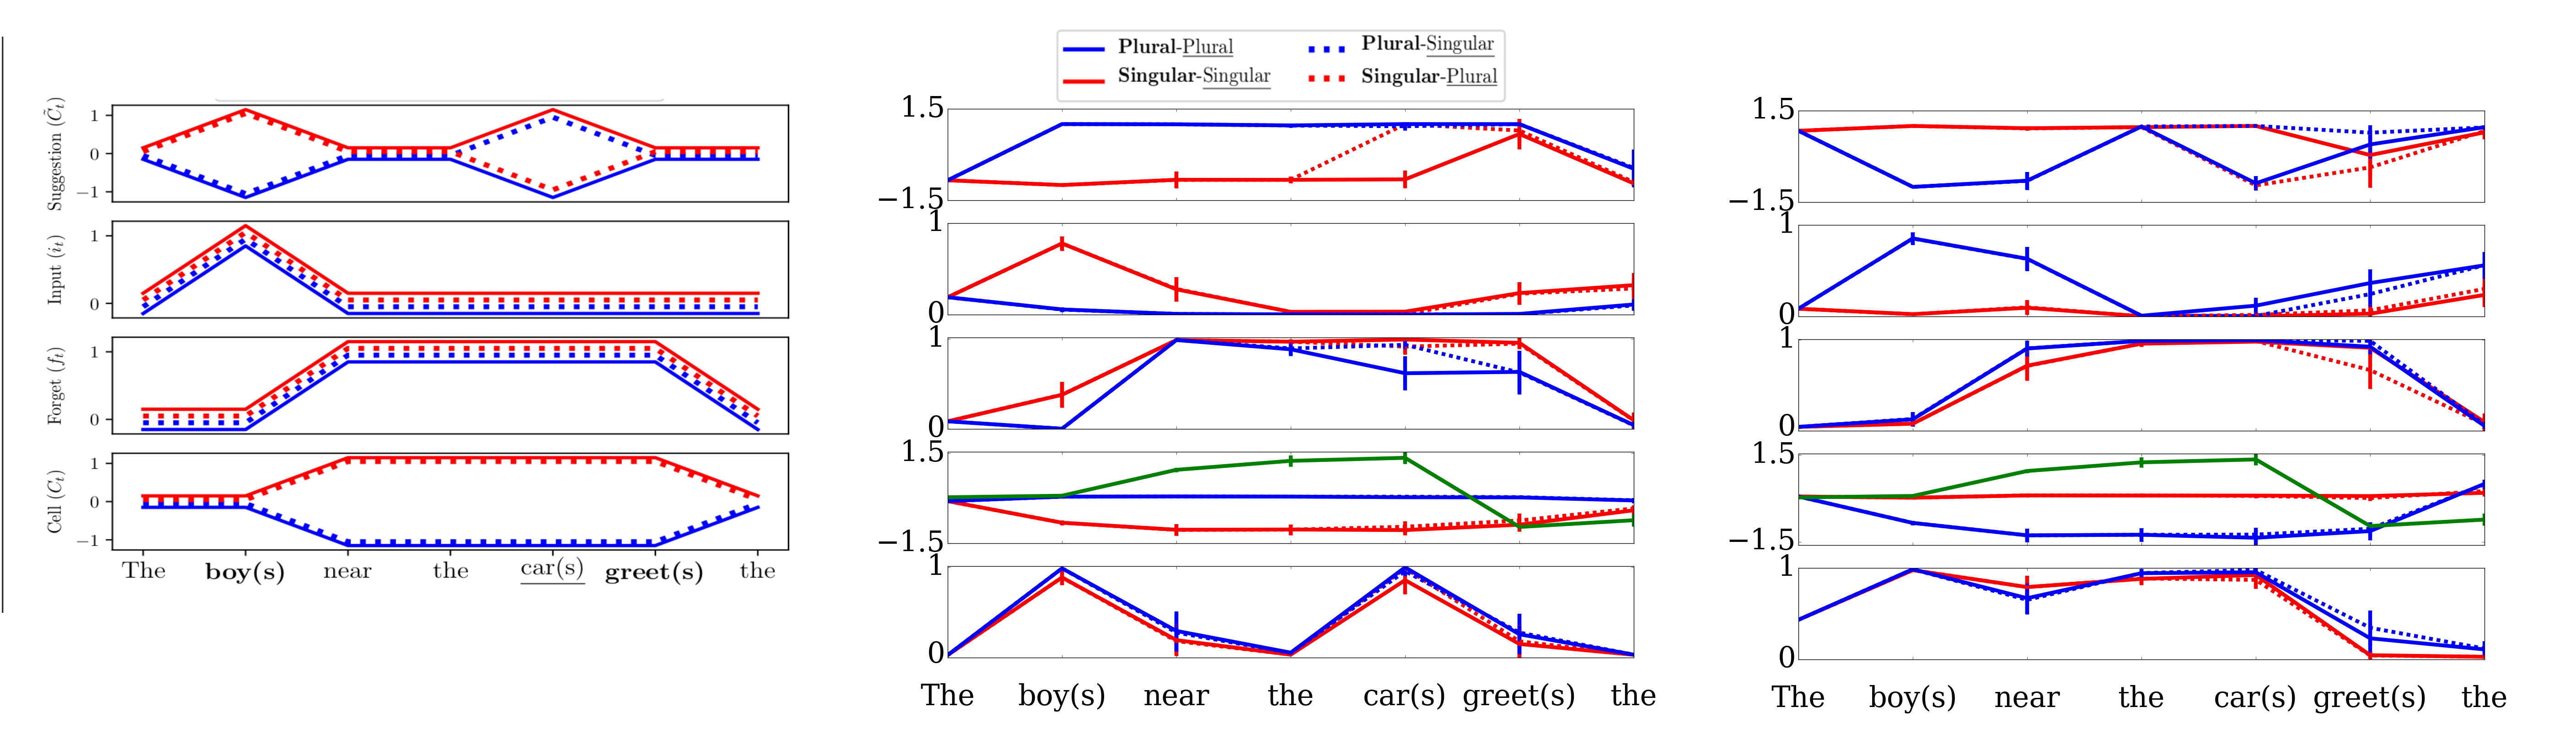
\includegraphics[width=\textwidth]{Figures/Figure2_cartoon_LR_units.png}
    \centering
    \begin{subfigure}{\textwidth}
            \centering
            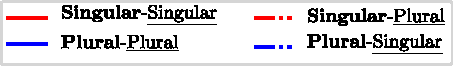
\includegraphics[width=0.3\linewidth]{Figures/legend.pdf}
    \end{subfigure}
    \bigskip
    \begin{subfigure}{0.3\textwidth}
            \centering
            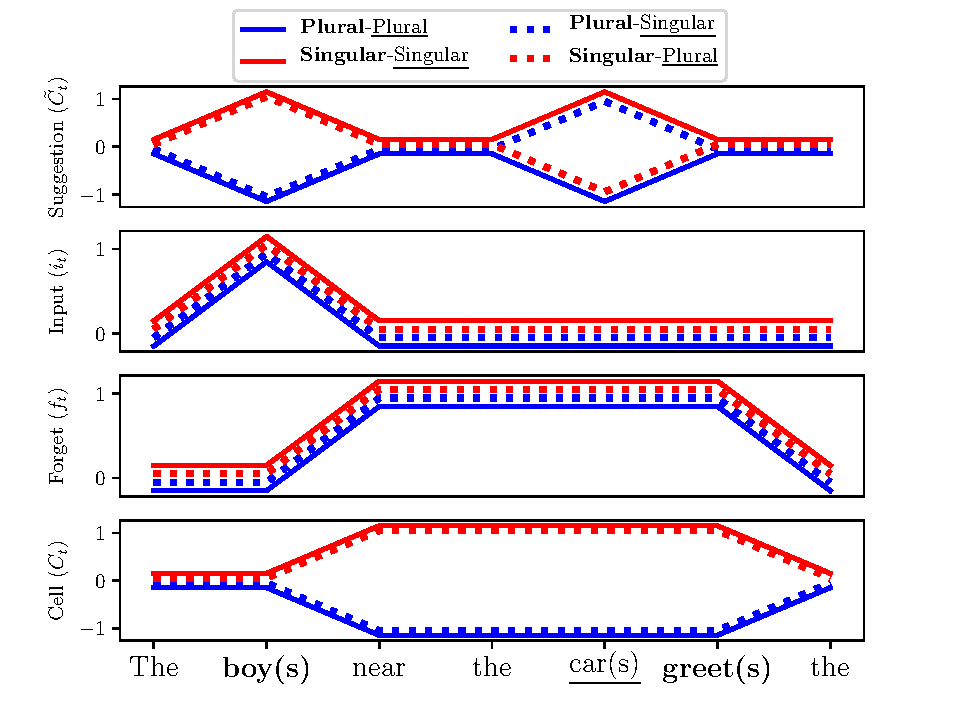
\includegraphics[width=\linewidth]{Figures/unit-timeseries-cartoon.pdf}
            \subcaption{Prediction (singular)}
    \label{fig:cartoon}
    \end{subfigure}
    \begin{subfigure}{0.3\textwidth}
            \centering
            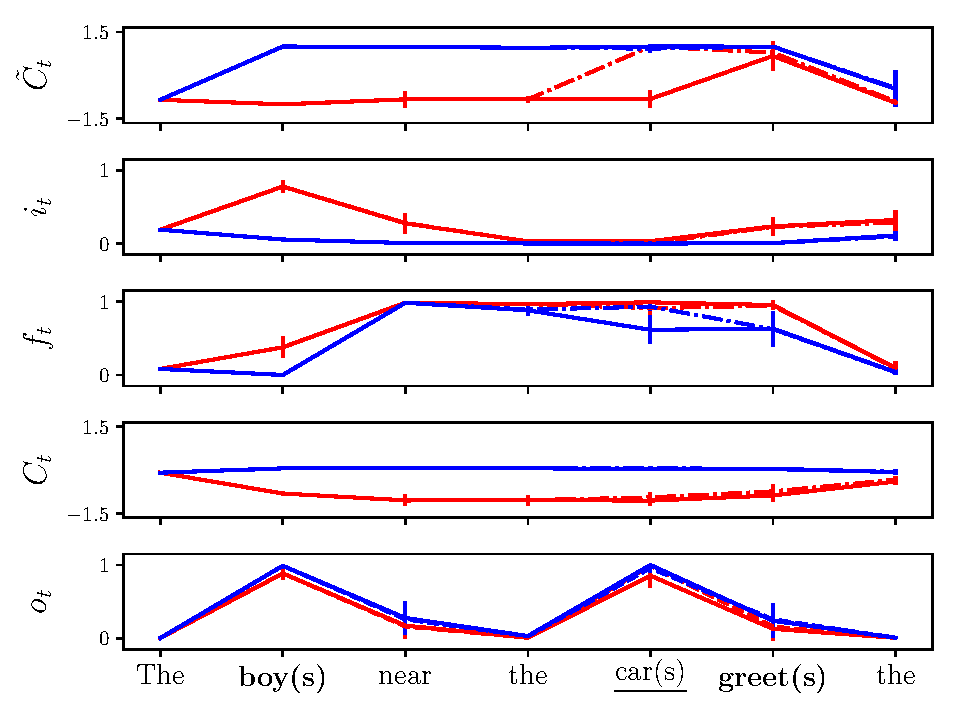
\includegraphics[width=\linewidth]{Figures/nounpp_987.pdf}
            \subcaption{Unit 998 (singular)}
    \label{fig:singular-unit}
    \end{subfigure}
    \begin{subfigure}{0.3\textwidth}
            \centering
            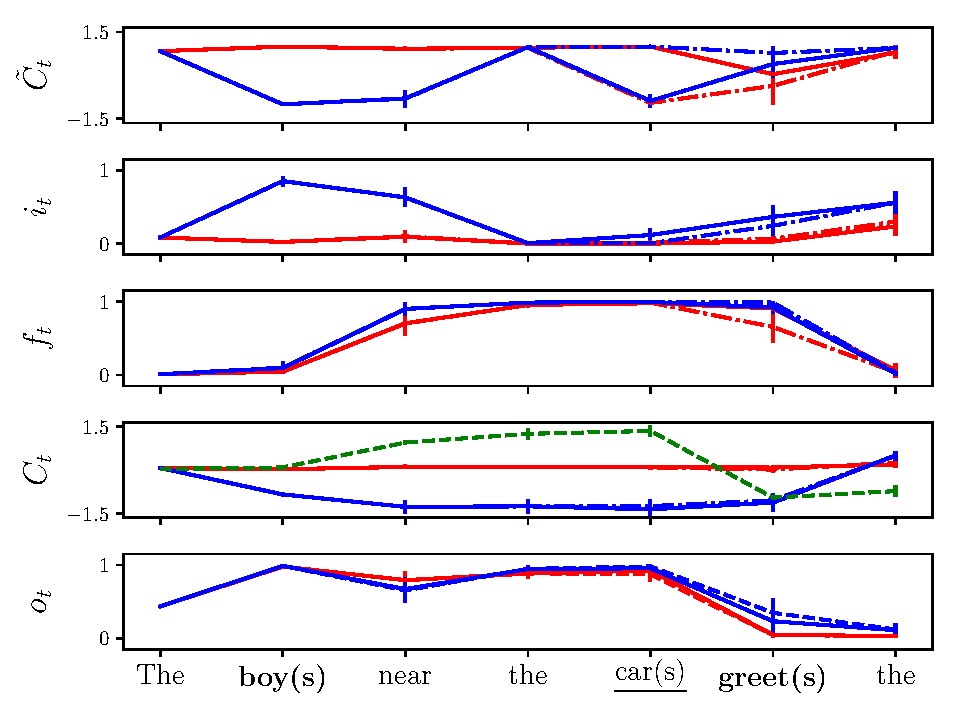
\includegraphics[width=\linewidth]{Figures/nounpp_775.pdf}
            \subcaption{Unit 776 (plural)}
    \label{fig:plural-unit}
    \end{subfigure}
\caption{Cell and gate activations during processing of a sentence with a prepositional phrase between subject and verb.}
\end{figure*}

To understand the underlying mechanism of the singular and plural units, we now look into gate and state dynamics of these units during sentence processing. We focus on the nounPP NA-task, which is the simplest NA-task with a long-range dependency having an interfering noun. 

To anticipate the results, we first discuss how a number unit may reliably encode and store subject number across interfering nouns. Figure\ref{fig:cartoon} exemplifies this for a singular unit, showing the desired gate and cell dynamics. The four conditions are represented with separated curves - red for singular subject, blue for plural, and dashed lines for incongruent conditions. Gate and cell activity during times points that are unrelated to solving the NA-task are masked with white. We recall that the update rule of the LSTM cell has two terms Eq.\ref{eq:update-rule}: in the first, $f_t * C_{t-1}$, the forget gate controls whether to keep the previous cell content ($f_t=1$ - perfect remembering) or forget it ($f_t=0$ - complete forgetting). In the second term, $i_t*\tilde{C}_t$, the input gate controls whether the information currently presented to the network as encoded by $\tilde{C}_t$ can update onto the cell ($i_t=1$ - full access) or not ($i_t=0$). The singular unit can thus use these gates to reliably store number information across long-range dependencies. Specifically, the unit can: (1) encode subject number via $\tilde{C}_{t_{subject}}$ with different values for singular and plural; (2) open the input gate \textit{only} when a singular subject is presented ($i_t=1$ - red curves \textit{only}) and protect it from interfering nouns ($i_t=0, t<t_{verb}$); (3) while at the same time, clear the cell from previously stored information ($f_{t_{subject}}=0$) and then store subject number across the entire dependency ($f_t=1, t_{subject}<t<t_{verb}$); (4) Finally, output subject number at the right moment, when predicting verb form $o_{t_{verb}-1}=1$ (Eq.\ref{eq:output}). 

Figures \ref{fig:singular-unit} and \ref{fig:plural-unit} present the actual gate and cell dynamics of the singular and plural units. Error-bars represent standard deviation across all condition sentences. Results show that both units follow the general solution for reliable number storage described above. Note that the plural unit 'mirrors' the solution with respect to subject number (PP and PS vs. SS and SP), which is in accordance with the results of the ablation experiments that showed effect for only one value of subject number (table \ref{tab:ablation-results}). Taken together, it clarifies why ablating either one of these two units can bring the network to around chance-level performance in incongruent conditions - without the stored number information in the cell of these number units the network hopelessly tries to solve the NA-task.

A single divergence between the solution depicted in figure \ref{fig:cartoon} and the actual dynamics of the number units, is that input-gate activity is smaller, but not zero, at the time step immediately following the subject. This requires further research but one speculative explanation for this is that this behavior is required for the case of compound nouns. In these cases, subject number resides at the second noun, whereas in the case of simple nouns there is no 'risk' of encountering an interfering noun immediately after the subject. 

\subsubsection{Predicting the verb form}\label{subsec:output-weight}
\begin{figure*}[t!]
    \centering
    % GAT
    \begin{subfigure}{0.45\textwidth}
            \centering
            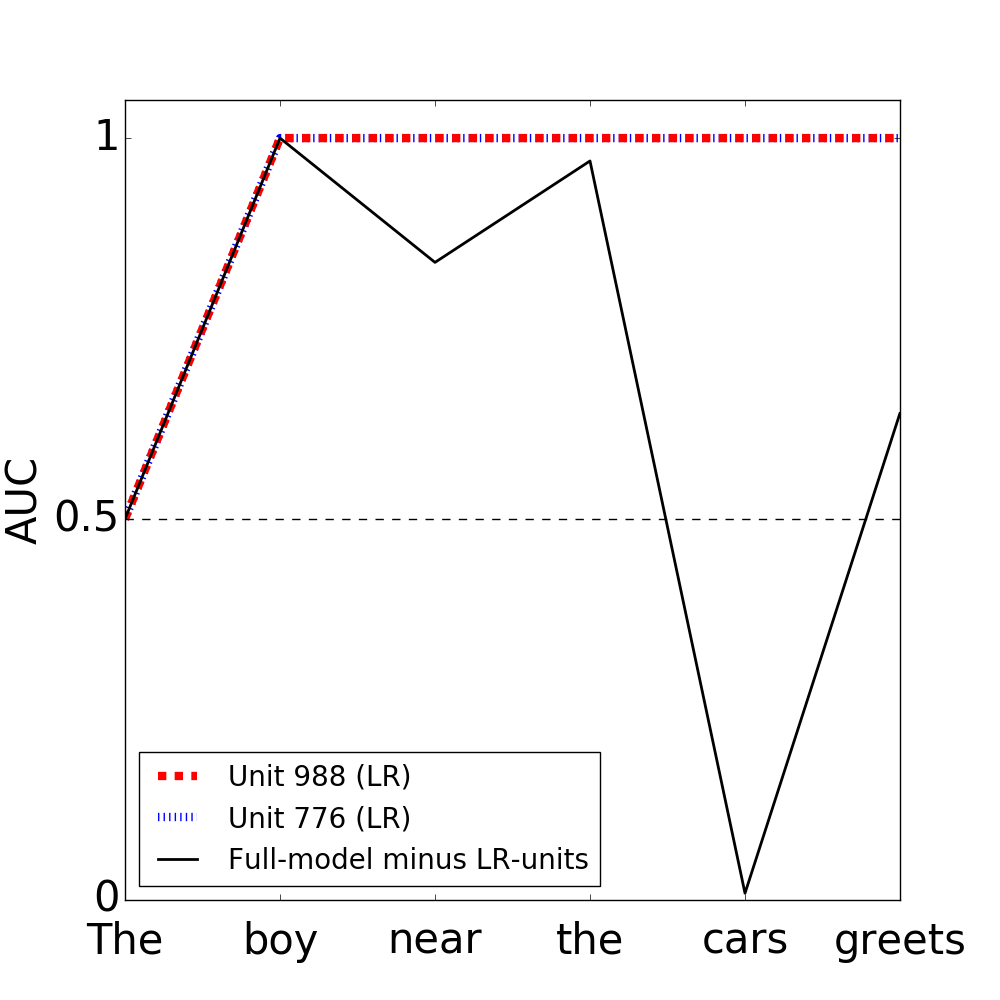
\includegraphics[height=5cm]{Figures/GAT1d_cell_nounpp_SR_LR_single_unit.png}
            \subcaption{Generalization across time.}
            \label{fig:GAT}
    \end{subfigure}
    \begin{subfigure}{0.45\textwidth}
            \centering
            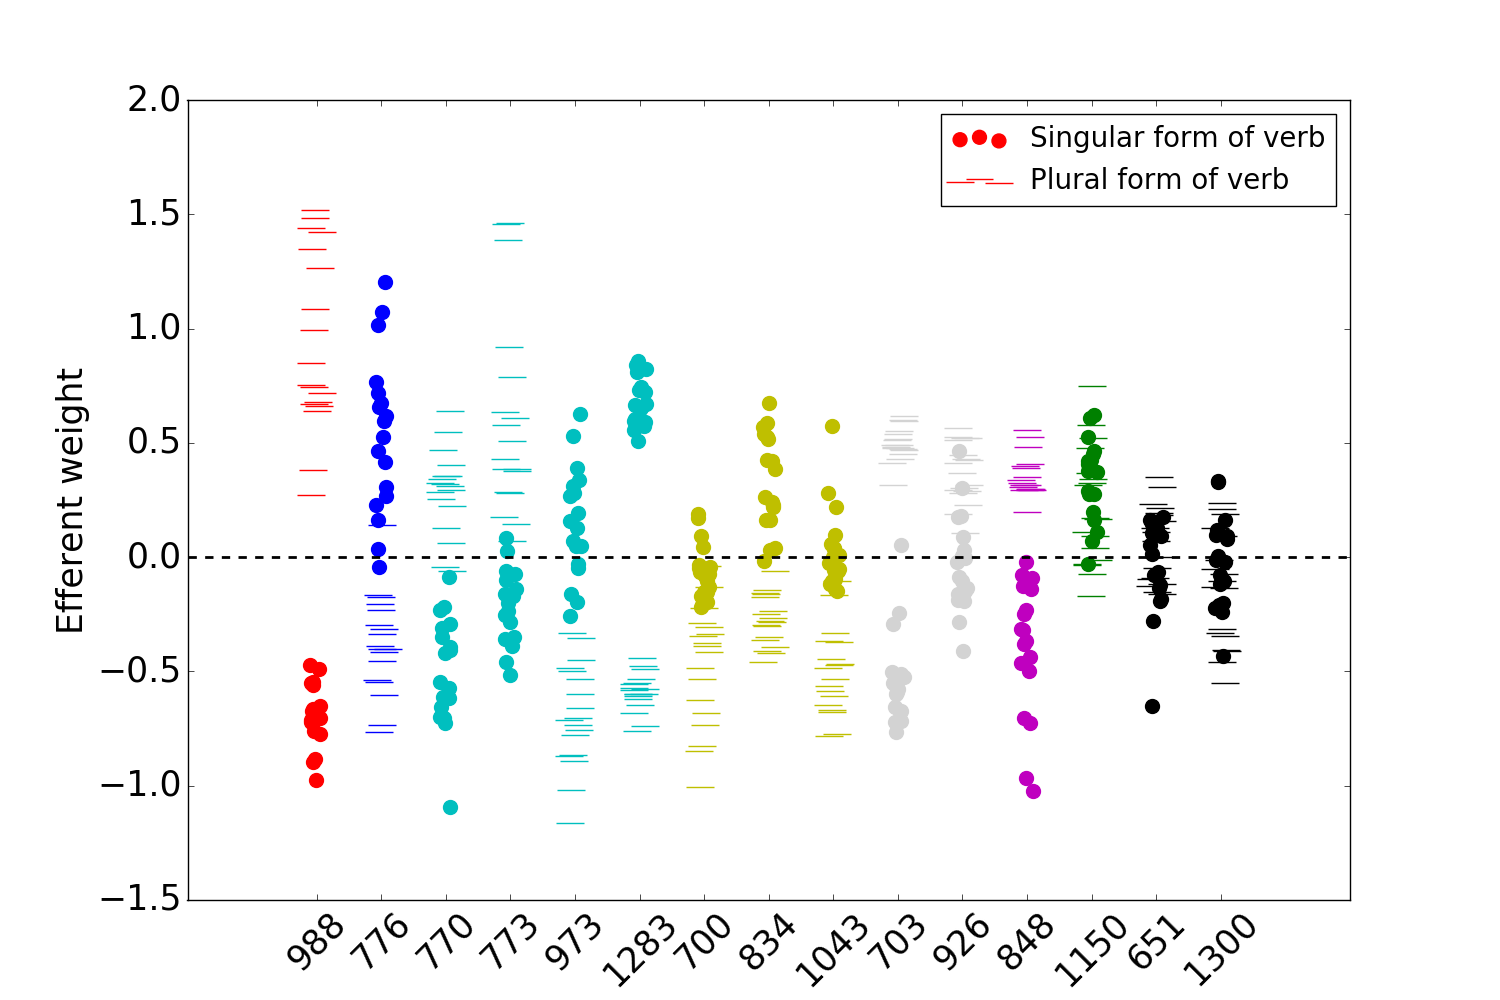
\includegraphics[height=5cm]{Figures/Figure5_output_weights.png}
            \subcaption{Efferent weights of number units.}
            \label{fig:output-weights}
    \end{subfigure}
    
%\caption{(A) Generalization across time of network units. (B) Output weights of SR units, LR units, syntax unit, and two arbitrary units.}
\end{figure*}

The singular and plural units have emerged at the second layer of the network. This seems appropriate if number information needs to be directly projected to the output layer for correct verb-form prediction. Moreover, it seems required that the output from the number units will be projected differently to singular and plural verb forms in the output layer, such that it will increase activity only in units representing the suitable form. For example, for the singular unit, since singular subjects are encoded with a negative value ($C_{t_{verb}-1}<-1$ in figure \ref{fig:singular-unit}), the more negative its efferent weights to singular verb forms at the output layer are the higher the probabilities of these verb forms would be. Extracting the efferent weights of the number units to all verbs in our dataset, we find that the efferent weights to the singular and plural verb forms are indeed segregated from each other \yair{singular unit: mean + std to plural, and mean+std to singular; plural unit: mean + std to plural, and mean+std to singular}, with weight signs that correspond to the negative encoding of subject number used by both singular and plural units. 

\subsubsection{Short-range number units}
Performance on several NA-tasks (Simple, Adv, 2Adv) was not impaired by single-unit ablations in any of their conditions. This suggests that subject number may be encoded also elsewhere in the network, perhaps via a more distributed code \marco{Cite Dieuwke's paper on this.}. To identify such other number units, we tested whether subject number can be decoded from the activity of units in the network, whether this decoding is stable during succeeding time points, and whether the efferent weights of the most informative units about subject number are segregated as those of the LR-number units. 

For each unit, we trained a linear model to predict subject number of the incongruent conditions based on cell activity during the presentation of the subject, and tested its prediction on test sets from all time points \yair{cite King and Dehaene}, using the Area under of Curve (AUC) to evaluate model performance. To quantify to what extent the efferent weights of each unit are segregated with respect to singular and plural verb forms, we used the statistical distance: $d^u_{W_P, W_S}=\frac{|\bar{W_S}-\bar{W_P}|}{\sigma_S+\sigma_P}$, where $W_S, W_P$ are the two sets of weights to singular and plural verb forms of unit $u$ with means $\bar{W_S}, \bar{W_P}$ and standard deviations $\sigma_S, \sigma_P$. 

Figure \ref{fig:GAT} shows the decoding across time from units with both AUC values and $d^u_{W_P, W_S}$ within the top five percentile across all units. Figure \ref{fig:output-weights} presents the corresponding efferent-weight distributions from all number units, including the singular and plural units, and two arbitrary non-number units (units \unit{2}{1} and \unit{2}{650}). These results suggests that subject number is distributively encoded by the network for short-range dependencies without interfering nouns, and locally for LR dependencies with such interfering nouns. \yair{todo: clean GAT plot based on also the nounPPadv task}